\section{Singular Value Decomposition}
The Singular Value Decomposition (SVD) is a matrix factorization with guaranteed existence.
It can be used to obtain low-rank approximations of a matrix or pseudo inverses for an ill-posed linear system of equations.
It is also related to FT by providing a data-specific set of orthogonal bases instead of a generic set of sines and cosines. For this paper, the SVD will be used for generating low-rank approximations of matrices \cite{brunton_kutz_2019b}.
\subsection{Properties}
A matrix \(X \in \mathbb{R}^{n \times m}\) can be decomposed in the following way
\begin{gather}
X = U \Sigma V^{T} \,.
\end{gather}
Here \(U \in\mathbb{R}^{n \times n}\) and \(V \in\mathbb{R}^{m \times m}\) are unitary matrices and \(\Sigma \in \mathbb{R}^{n \times m}\) is a real valued ordered diagonal matrix.
The columns of \(U\) provide a set of orthonormal basis vectors for the column space of \(X\), and \(V\) contains orthonormal basis vectors for the row space of \(X\). The matrix \(\Sigma\) assigns a magnitude ('importance') to the product of \(U\) and \(V^{T}\)  \cite{brunton_kutz_2019a}.
Since \(U\) and \(V\) are unitary they have the following property \cite{SZABO2015385}
\begin{gather}
U^{T}U = UU^{T} = I \\
V^{T}V = VV^{T} = I \,.
\end{gather}

In case \(n \geq m\), the so-called economy SVD can be used to factorize the matrix \(X\)
\begin{gather}
X = \begin{bmatrix}
\hat{U} & \hat{U}^{\bot}
\end{bmatrix} 
\begin{bmatrix}
\hat{\Sigma} \\
0
\end{bmatrix}
V^{T} = \hat{U} \hat{\Sigma} V^{T} \,.
\end{gather} 
The economy SVD omits rows only containing zeros in \(\Sigma\) and the according columns of \(U\).
Therefore the dimensionality of \(\hat{U}\) and \(\hat{\Sigma}\) is less or equal to the dimensionality of \(U\) and \(\Sigma\) 
 \cite{brunton_kutz_2019b}.

\subsection{Hierarchy of Correlations}
As already stated, the matrix \(\Sigma\) assigns a magnitude to \(UV^{T}\).
This magnitude is the square of the variance of the bases in \(U\) and \(V\) capture.
Assume that \(X^{T}X\) and \(XX^{T}\) denote correlation matrices
\cite{brunton_kutz_2019b}.
A correlation matrix is a matrix that stores correlation coefficients between multiple measurements. 
If \(X\) has the following properties \(X^{T}X\) and \(XX^{T}\) are correlation matrices.
\paragraph{1.) The column vectors of \(X\) have to be zero mean}
\begin{gather}
X = \begin{bmatrix}
x_1 & \hdots & x_m
\end{bmatrix} \\
\frac{1}{n}\sum_{i = 1}^{n} x_{ij} = \mu_{i} = 0 \quad , 1 \leq i \leq m \,.
\end{gather}
\paragraph{2.) The column vectors of \(X\) have to be normalized}
\begin{gather}
\sqrt{\sum_{i = 1}^{n} x_{ij}^{2}} = \bar{x_i} = 1 \quad , 1 \leq i \leq m \,.
\end{gather}
The correlation coefficient between two column vectors of \(X\) is calculated as follows \cite{Suga}
\begin{gather}
\operatorname{corr}(x_i, x_{i'})\frac{(\sum_{j = 1}^{n} x_{ij} - \bar{x}_i)(\sum_{j = 1}^{n} x_{i'j} - \bar{x}_{i'})}{(\sum_{j = 1}^{n} (x_{ij}- \bar{x_{i}})^{2})^{\frac{1}{2}}(\sum_{j = 1}^{n} (x_{i'j}-  \bar{x}_{i'})^{2})^{\frac{1}{2}}} \,.
\end{gather}



Since all column vectors have zero means and are normalized, this becomes \cite{harv}
\begin{gather}
\operatorname{corr}(x_i, x_{i'}) = cov(x_i, x_{i'})= x_i^{T}x_{i'} \,.
\end{gather}

This resembles the entries of \(XX^{T}\) and \(X^{T}X\).
A vector \(e\) that maximizes the variance of the projection of \(x_i\) onto \(e\)  with the restriction \(||e|| = 1\) are the eigenvectors of the according correlation matrix.
The eigenvalue of \(e\) denoted as \(\lambda\) is equivalent to the variance of \(x_i\) projected onto \(e\) \cite{Lavrenko}.

Since \(X\) can be de-constructed using the SVD, \(XX^{T}\) and \(X^{T}X\) are equal to
\begin{gather}
XX^{T} = U\begin{bmatrix}
\hat{\Sigma} \\
0
\end{bmatrix}V^{T}V\begin{bmatrix}
\hat{\Sigma} & 0
\end{bmatrix}U^{T} = U \begin{bmatrix}
\hat{\Sigma}^{2} & 0 \\
0 & 0
\end{bmatrix} U^{T} \label{corr-1}\\
X^{T}X = V \begin{bmatrix}
\hat{\Sigma} & 0
\end{bmatrix} U^{T}U \begin{bmatrix}
\hat{\Sigma} \\
0
\end{bmatrix} V^{T} = V\hat{\Sigma}^{2}V^{T} \,. \label{corr- 2}
\end{gather}
By multiplying \(U\) and \(V\) respectively on the right side (\ref{corr-1}) and (\ref{corr- 2}) become
\begin{gather}
XX^{T}U = U \begin{bmatrix}
\hat{\Sigma}^{2} & 0 \\
0 & 0
\end{bmatrix} \\
X^{T}XV = V\hat{\Sigma}^{2} \,.
\end{gather}
This shows that \(V\) contains the eigenvectors of the row-wise correlation matrix, and \(U\) contains the eigenvectors of the column-wise correlation matrix.
The matrix \(\Sigma\) contains the roots of the according eigenvalues and is related to the variance.
By ordering \(U\), \(\Sigma\) and \(V\) by the entries of \(\Sigma\) in a descending order he first row of \(U\) and \(V\) contain the most important basis vectors \cite{brunton_kutz_2019b}.

\subsection{Low-rank Approximation}
A useful property of the SVD is that it can be used to find a hierarchy of rank-\(r\) approximations for a given matrix \(X\).
An matrix \(\tilde{X}\) that approximates \(X\) is obtained by 
\begin{gather}
\tilde{X} = \argmin\limits_{s.t. rank(\tilde{X}) = r} 
 ||X - \tilde{X}||_F = \tilde{U}\tilde{\Sigma}\tilde{V}^{T}
\end{gather}	
Here  \(\tilde{U}\) and \(\tilde{V}\) denote matrices obtained taking the first \(r\) columns of \(U\) and \(V\). The matrix \(\tilde{\Sigma}\) is a \(r \times r\) sub-block of \(\Sigma\).
This is also known as the Eckard-Young theorem.
The variance captured by \(\tilde{X}\) can be calculated in the following way \cite{brunton_kutz_2019b}
\begin{gather}
\operatorname{cumvar}_{r}(\Sigma) = \frac{\sum_{i = 1}^{r} \sigma_i}{\operatorname{trace}(\Sigma)} \label{cum-var-r} \\
\operatorname{var}(\Sigma) = \frac{\operatorname{diag}(\Sigma)}{\operatorname{trace}(\Sigma)} \,. \label{var-sig}
\end{gather}

\subsection{Example low-rank Approximation}
As an example, suppose there is a matrix \(X\)
\begin{gather}
X = \begin{bmatrix}
3 & 1 & 5 & 5 \\
4 & -4 & 5 & 0 \\
-4 & -2 & -4 & 3 \\
5 & 1 & 5 & -4
\end{bmatrix} \,.
\end{gather}
By computing the SVD the matrices \(U\), \(\Sigma\) and \(V\) are obtained.
Now \(\Sigma\) can be used to calculate the cumulative variance for a rank-\(r\) approximation and the variance captured by each basis vector of \(U\) and \(V\).
\pgfplotsset{width=6cm,compat=1.9}
\begin{figure}[H]
\centering
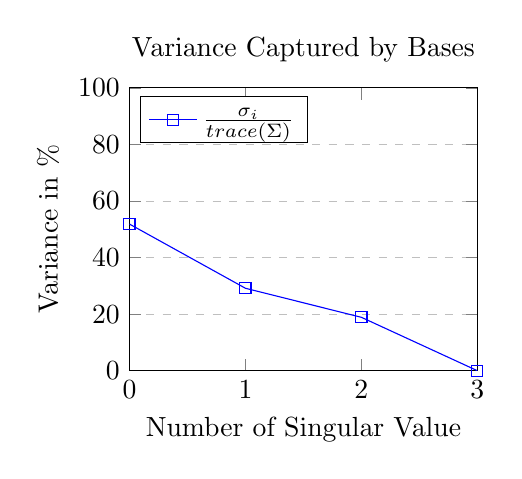
\begin{tikzpicture}
\begin{axis}[
    title={Variance Captured by Bases},
    xlabel={Number of Singular Value},
    ylabel={Variance in \%},
    xmin=0, xmax=3,
    ymin=0, ymax=100,
    xtick={0,1,2,3},
    ytick={0,20,40,60,80,100},
    legend pos=north west,
    ymajorgrids=true,
    grid style=dashed,
]

\addplot[
    color=blue,
    mark=square,
    ]
    coordinates {
    (0,51.87)(1,29.18)(2,18.91)(3,0.04)
    };
    \legend{\(\frac{\sigma_{i}}{trace(\Sigma)}\)}
    
\end{axis}
\end{tikzpicture}
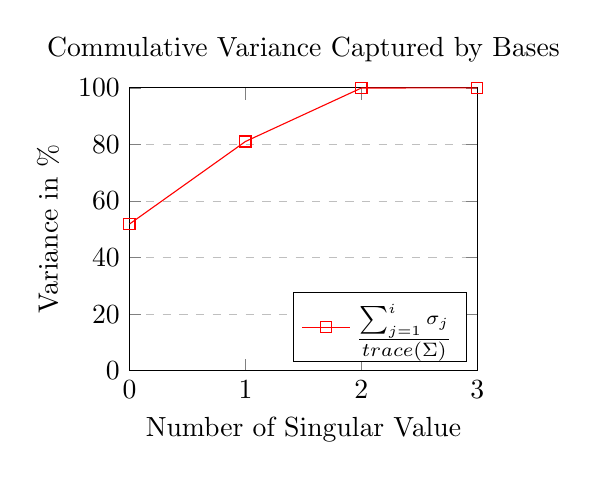
\begin{tikzpicture}
\begin{axis}[
    title={Commulative Variance Captured by Bases},
    xlabel={Number of Singular Value},
    ylabel={Variance in \%},
    xmin=0, xmax=3,
    ymin=0, ymax=100,
    xtick={0,1,2,3},
    ytick={0,20,40,60,80,100},
    legend pos=south east,
    ymajorgrids=true,
    grid style=dashed,
]
\addplot[
    color=red,
    mark=square,
    ]
    coordinates {
    (0,51.87)(1,81.05)(2,99.96)(3,100)
    };
    \legend{\(\frac{\sum_{j=1}^{i}\sigma_{j}}{trace(\Sigma)}\)}

\end{axis}
\end{tikzpicture}
\caption{Variance and cumulative variance captured by each column vectors of \(U\) and \(V\)}
\label{var-plt}
\end{figure}
In figure \ref{var-plt}, the commutative variance and the variance of each basis vector are plotted.
Here \(X\) can be approximated using the first three leading basis vectors.
This approximation captures already more than 99\% of the variance.
The resulting matrix \(\tilde{X}_3\) looks as follows
\begin{gather}
\tilde{X}_3 = \begin{bmatrix}
4.73 & -0.76 & 5.62 \\
1.31 & -1.37 & 1.62 \\
-5.10 & -0.60 & 2.34
\end{bmatrix} \,.
\end{gather}





